\section{Background}
\label{sec:background}
Among the most important web metrics are load times, number \& size of objects, and page size. Each of the aforementioned metrics can be measured according to numerous definitions and using data from diverse data sources. The following section provides an overview of these definitions and the data sources used in this paper.

\subsection{Load Times}
The time required for loading a web page correlates strongly with user experience \cite{6263888}. A browser normally loads a web page in multiple steps: load and parse the base document, construct a Document Object Model (DOM), load and process referenced objects, render / display the results. Although Page Load Time (PLT), defined as the time until the onLoad event, is most often used to measure page load times, there are a number of other metrics. For example, Time To First Paint (TTFP) and Above The Fold Time (AFT) are triggered before PLT when the content is first displayed and available to the user. The start times used for calculating load times can always differ (e.g. navigationStart, fetchStart). One of the main takeaways from \cite{10.1007/978-3-030-15986-3_19} is that redirects can strongly affect these measurements and should be accounted for; Figure \ref{fig:plot_redirects} shows the impact redirects can have on PLT and Figure \ref{fig:bar_redirects} the prevalence of such redirects. 

There is also a plurality of data sources for calculating load times. The standardized API for navigation timings \cite{timing_2012} is used to fetch load times based on browser events. It is important to note that events / metrics provided by the Navigation Timings API are not necessarily defined in the same way for all browsers. HTTP Archive files \cite{har_format_2012} and the Resource Timings API \cite{w3c_2020} also provide load time data. The majority of modern browsers (e.g. Chrome, Firefox) implement the Navigation Timings and Resource Timings APIs; HAR files can be exported using developer tools. Both Chrome and Firefox provide remote debugging and page load automation interfaces (i.e. Chrome DevTools \& Firefox Marionette). There are also third-party automation frameworks that allow for the same basic functionality as well as extended functions (e.g. keyboard input); Selenium, one of the most popular such tools, is used in the original paper.

 \begin{figure}
 \centering
 \begin{subfigure}{\linewidth}
		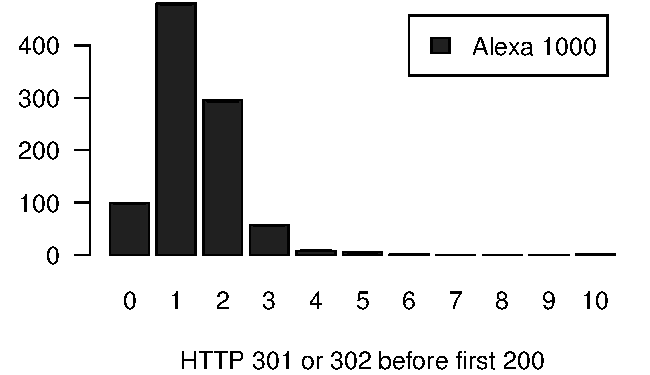
\includegraphics[width=\linewidth]{New_Plots/barplot_redirects_clean.pdf}
	\caption{New Measurements}
	\label{fig:new_bar_redirects}
\end{subfigure}\par\medskip
\begin{subfigure}{\linewidth}
		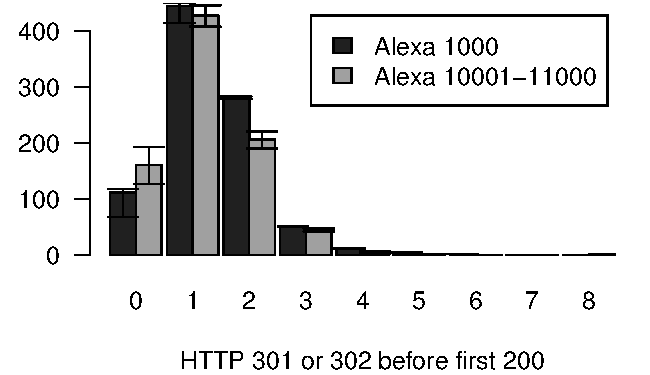
\includegraphics[width=\linewidth]{Original Plots/barplot_redirects.pdf}
	\caption{Original Measurements}
	\label{fig:orig_bar_redirects}
\end{subfigure}
\caption{Number of initial Redirects}
\label{fig:bar_redirects}
\end{figure}

\begin{figure}
 \centering
 \begin{subfigure}{\linewidth}
		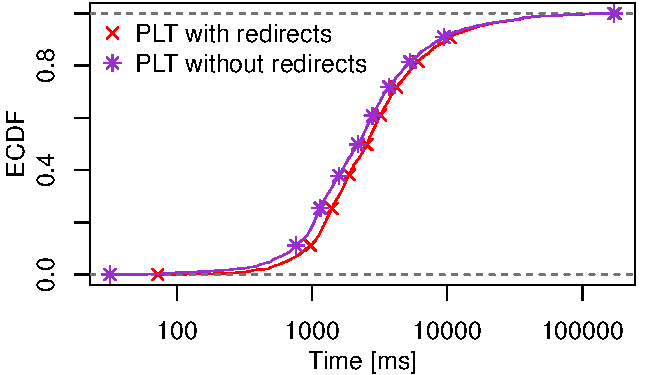
\includegraphics[width=\linewidth]{New_Plots/ecdf_loadtimes.pdf}
	\caption{New Measurements}
	\label{fig:new_plot_redirects}
\end{subfigure}\par\medskip
\begin{subfigure}{\linewidth}
		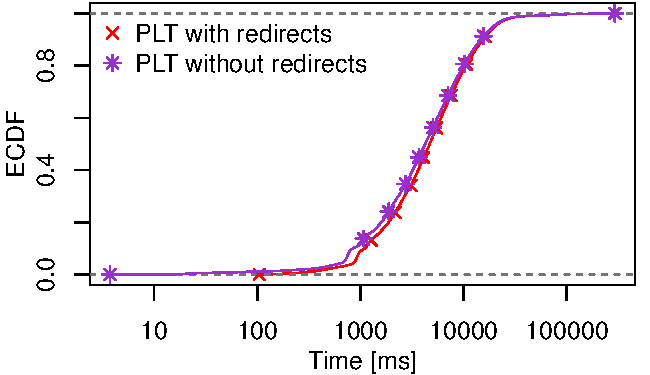
\includegraphics[width=\linewidth]{Original Plots/ecdf_loadtimes.pdf}
	\caption{Original Measurements}
	\label{fig:orig_plot_redirects}
\end{subfigure}
\caption{Page Load Time (PLT) with and without initial redirects}
\label{fig:plot_redirects}
\end{figure}

\subsection{Number and Size of Objects}
In order to estimate the complexity of web pages, metrics such as Object Index, Object Count, and Byte Index are employed. Since web pages are often constantly loading - even after the initial page load - object counts should only count objects loaded by the onLoad event. Calculating a count of the initial objects can be done using objects in the DOM or HTTP request-response pairs. Object size normally reflects the encoded size (i.e. the count of bytes transferred over the network) but can also reflect the decoded (i.e. decompressed) number of bytes. Byte Index refers to the integral of the total sizes of objects loaded over time and is an important metric for the size of Objects \cite{10.1145/2940136.2940138}.

To obtain the number of objects, one can count the number of HTTP request-response pairs in HAR files. The number of objects can also be obtained using the Resource Timings API. Both the Resource Timings API and HAR files supply the encoded and decoded body size. Alternatively, the number of objects can be extracted from packet capture traces if all elements can be decrypted; if this is not the case, object sizes can differ due to TLS padding.